\documentclass[review]{elsarticle}

\usepackage{lineno,hyperref}
\usepackage[ruled]{algorithm2e}
\usepackage{subfigure}
\usepackage{amsmath}
%\usepackage{algorithm}
\usepackage{algorithmic}
\usepackage{multirow}
\renewcommand{\algorithmcfname}{ALGORITHM}
\renewcommand{\algorithmicrequire}{\textbf{Input:}} % Use Input in the format of Algorithm
\renewcommand{\algorithmicensure}{\textbf{Output:}} % Use Output in the format of Algorithm
\SetAlFnt{\small}
\modulolinenumbers[5]

\usepackage{color}
\newcommand\revised[1]{{\color{black} #1}}
\journal{Expert Systems with Applications}

%%%%%%%%%%%%%%%%%%%%%%%
%% Elsevier bibliography styles
%%%%%%%%%%%%%%%%%%%%%%%
%% To change the style, put a % in front of the second line of the current style and
%% remove the % from the second line of the style you would like to use.
%%%%%%%%%%%%%%%%%%%%%%%

%% Numbered
%\bibliographystyle{model1-num-names}

%% Numbered without titles
%\bibliographystyle{model1a-num-names}

%% Harvard
%\bibliographystyle{model2-names.bst}\biboptions{authoryear}

%% Vancouver numbered
%\usepackage{numcompress}\bibliographystyle{model3-num-names}

%% Vancouver name/year
\usepackage{numcompress}\bibliographystyle{model4-names}\biboptions{authoryear}

%% APA style
%\bibliographystyle{model5-names}\biboptions{authoryear}

%% AMA style
%\usepackage{numcompress}\bibliographystyle{model6-num-names}

%% `Elsevier LaTeX' style
%\bibliographystyle{elsarticle-num}
%%%%%%%%%%%%%%%%%%%%%%%

\begin{document}
	
	\begin{frontmatter}
		
		\title{A Learnable Search Result Diversification Method}
		%\tnotetext[mytitlenote]{Fully documented templates are available in the elsarticle package on \href{http://www.ctan.org/tex-archive/macros/latex/contrib/elsarticle}{CTAN}.}
		
		%% Group authors per affiliation:
		
		\author[mymainaddress,htemail]{Hai-Tao Zheng\corref{mycorrespondingauthor}}
		\cortext[mycorrespondingauthor]{Corresponding author}
		
		\author[mymainaddress,jxemail]{Jinxin Han}
		\author[mymainaddress,zremail]{Zhuren Wang}
		\author[mymainaddress,xxemail]{Xi Xiao}
		
		\address[mymainaddress]{Tsinghua-Southampton Web Science Laboratory, Graduate School at Shenzhen, Tsinghua University, China}
		\address[htemail]{zheng.haitao@sz.tsinghua.edu.cn}
		\address[jxemail]{hanjx16@mails.tsinghua.edu.cn}
		\address[zremail]{wang-zr14@mails.tsinghua.edu.cn}
		\address[xxemail]{xiaox@sz.tsinghua.edu.cn}


\begin{abstract}
\indent Search result diversification is to tackle the ambiguous queries and multi-faced information needs. The search result diversification problem can be formalized as a balance between the relevance score and the diversity score. Most previous diversification models utilize a predefined function to calculate the diversity score. The values of parameters need to be tuned by manual experiments. It is time-consuming and hard to reach optimal result in diversity evaluation. Proposing a learnable approach to solve the above problems is a pressing task. Therefore we introduce a Learnable Search Result Diversification model called L-SRD. On this basis, we redefine the diversity function and derive our loss function as the likelihood loss of ground truth generation. Stochastic gradient descent algorithm is employed to optimize the values of parameters. Finally we derive our ranking function to generate the diverse list sequentially. Due to the learning model, the values of parameters are determined automatically and get optimally. The experiments on TREC web tracks show that our approach outperforms several existing diversification models significantly.
\end{abstract}

\begin{keyword}
Explicit Search Result Diversification\sep Learning Model \sep Markov Random Fields
\MSC[2017] 00-01\sep  99-00
\end{keyword}

\end{frontmatter}

\linenumbers


%\begin{abstract}
%% Search result diversification has been proposed to tackle the ambiguous queries and multi-faced information needs. The search result diversification problem can be formalized as a balance between relevance score and diversity score. Most previous diversification models utilize a predefined function to calculate the diversity score. It is subjective and hard to reach optimal result. Meanwhile, the value of parameters need to be tuned manually by the repeat experiment, which is aimless and gives rise to a time-consuming problem. To address these issues, we introduce a Markov Random Field based learning approach for search result diversification model called L-SRD.
%% %We extract a series of features on the basis of the Markov Random Field, enabling the integration of various type of features.
%% On this basis, we redefine the diversity function and derive our loss function as the likelihood loss of ground truth generation. Stochastic gradient descent are employed to optimize the value of features. Finally we derive our ranking function to generate the diverse list sequentially.
%% Benefit from the learning model, the parameter values are determined automatically and are optimal. %The experiments on TREC web tracks show that our method improves the query aspect diversification methods significantly.
%% The experiments on TREC web tracks show that our approach outperforms several existing diversification models significantly.
%
%Search result diversification has been proposed to tackle the ambiguous queries and multi-faced information needs. The search result diversification problem can be formalized as a balance between relevance score and diversity score. Most previous diversification models utilize a predefined function to calculate the diversity score. The value of parameters need to be tuned manually by the repeat experiment. It is time-consuming and hard to reach optimal result. Promising a learnable approach to solve parameter tuning problem and achieve optimal result in diversity evaluation is a pressing task. We introduce a learnable search result diversification model called L-SRD. On this basis, we redefine the diversity function and derive our loss function as the likelihood loss of ground truth generation. Stochastic gradient descent are employed to optimize the value of features. Finally we derive our ranking function to generate the diverse list sequentially. Benefit from the learning model, the parameter values are determined automatically and are optimal. The experiments on TREC web tracks show that our approach outperforms several existing diversification models significantly.
%
%\end{abstract}

\section{Introduction}
There are many ambiguous queries in search system. The keyword \textbf{apple} may refer to the Apple, one of the most famous companies in the world, or the electronics Apple manufactures. It may be the most familiar fruit also. There are many aspects of information needs underlying a simple query. How to produce a good quality diverse result is our main concern. 


\revised{
	The existing diversification approaches have been categorized as either implicit approaches or explicit approaches. The implicit approaches assume each document representing its own aspect and promote diversity by selecting documents for different aspects based on the difference of their vocabulary \cite{carbonell1998use}. It is a less effective model for the reason that it cannot express the inherent meaning well \cite{agrawal2009diversifying,zhai2003beyond}. 
	The explicit approaches are proposed to overcome the weakness. They explicitly formalize the aspects underlying a query and select documents that cover different aspects. The xQuAD and PM2 are classic explicit models \cite{santos2010exploiting,dang2012diversity}.
	But they just utilize a predefined function to calculate the diversity score based on query aspects. It is subjective and hard to reach optimal result.}


In this paper, we treat the Query Aspect Diversification as a learning problem and propose a Learnable Search Result Diversification (L-SRD) method. We incorporate various features into diversity measurement based on the Markov Random Field (MRF), which enables the integration of various types of features. The values of parameters can be determined automatically, which saves the manual labour, and the parameters are more optimal. Firstly we redefine the diversity function and derive our loss function as the likelihood loss of ground truth generation. Then Stochastic gradient descent algorithm is employed to optimize the values of weights. Finally we derive our ranking function to generate the diverse list sequentially.

%On this basis, we redefine the diversity function and derive our loss function as the likelihood loss of ground truth generation. Stochastic gradient descent are employed to optimize the value of features. Finally we derive our ranking function to generate the diverse list sequentially.

We conduct a series of experiments to demonstrate that L-SRD is more effective than other diversification models in terms of the official evaluation metrics including $\alpha$-nDCG, ERR-IA, NRBP  and the classical diversification metrics such as Precision-IA and Aspect Recall \cite{clarke2008novelty,chapelle2009expected,clarke2009effectiveness}. Additionally, we get a remarkable performance in robust evaluation.

The main contributions of our work are listed as follows:
\begin{enumerate}
	\item L-SRD introduces the learning mechanism to the query aspect diversification model. We conduct inference for the loss function based on its sequential selection model, which solves the parameters tuning problem automatically at the same time.
	
	\item We utilize the Markov Random Field to integrate different types of features to address the diversity measurement problem for query aspect search result diversification.
	
	\item We propose a sequential prediction method, which selects the best document from candidate set by maximizing ranking score.
	
	\item We conduct extensive experiments to verify L-SRD achieve better performance comparing with the existing diversification methods.
\end{enumerate}

The remainder of this paper is organized as follows. Section \ref{sec_rel} introduces the current research situation on the search result diversification. Section \ref{sec_model} describes the definition of the loss function and the estimation of parameters. Sections \ref{sec_setup} and \ref{sec_expres} detail the experiments setup on the TREC web track and their evaluations. In Section \ref{sec_con}, we summarize our achievements and give future works.

\section{Related Work}\label{sec_rel}


\revised{
	Search result diversification has a wide range of applications, such as patent search \cite{Kim:2015:IPS:2808194.2809455}, legal information retrieval \cite{a10010022} and so on.
	The process of diversification can be characterized as a bidirectional optimization problem, in which one seeks to maximize the overall relevance of a document ranking to multiple query aspects, while minimizing its redundancy \cite{Santos:2010:EQR:1772690.1772780}. In particular, the existing approaches can be categorized as either implicit or explicit making a difference in how they account for the query aspects \cite{10.1007/978-3-642-12275-0_11}.
	}


\revised{
 The basic assumption of implicit diversification approaches is that dissimilar documents are more likely to satisfy different information needs. The most representative approach in maximal marginal relevance (MMR) method and its probabilistic variants is shown as follows \cite{zhai2003beyond}:
\begin{equation}
S_{MMR}(q,d,c) = (1-\lambda)S^{rel}(d,q) - \lambda \mathop{}_{d_j \in C}^{max}   S^{div}(d,d_{j})
\end{equation}
where $ S^{rel}  $and $ S^{div}  $ represents  document $d's$ relevance to the query $q$ and its similarity to a selected document $d_{j}$ respectively. To gain high ranking score, a document should not only be relevant, but also be dissimilar from the selected documents.
%Zhu et al. \cite{zhu2007improving} rank sentences using random walks in an absorbing Markov chain and model directed graphs based on the document link structure \cite{zhang2005improving}.
The special process of MMR proposed by Garbonell \& Goldstein is selecting the document iteratively \cite{carbonell1998use}, and meanwhile, both content-based relevance and diversity relation between current selected document and the previously selected documents are considered. Yu et al. formulate this as a process of selecting and ranking $k$ exemplar documents and utilize linear programming to solve this problem \cite{Yu:2017:CIL:3018661.3018710}.
In summary, they are all implicit approaches without using aspects to mine the underlying aspects, besides, they are a low effective approaches \cite{santos2010exploiting,drosou2010search}.


Explicit approaches make use of the aspects underlying the query to select documents that cover different aspects as far as possible. The algorithms such as IA-select \cite{agrawal2009diversifying}, xQuAD \cite{santos2010exploiting} and RxQuAD \cite{vargas2012explicit} are proposed to reduce redundancy on the aspect levels. These methods select documents that cover more novel aspects. The PM-1 and PM-2 models pay more attention to maintain the proportionality of aspects \cite{dang2012diversity}. They produce the ranked result according to the proportionality of aspects. Intrinsic diversity products a series of successor queries to figure out the appropriate content to cover \cite{raman2013toward}. \cite{Wang:2016:ESR:2911451.2911497} and \cite{Hu15searchresult} think the aspects underlying the query should be hierarchical, and propose some hierarchical measures to find the relationships among aspects. \cite{Ullah2016QuerySM} mine query subtopic by exploiting the word embedding and short-text similarity measure. 
To conclude, all existing explicit approaches are unsupervised, and the values of parameters need to be tuned by the experiment repeatedly without intention, causing a time-consuming optimizing problem to find the most suitable parameters.

%Yu et al.\cite{yu2014search} formulized the problem as a 0-1 multiple subtopic knapsack problem.


Some learning approaches are also proposed for search result diversification. For example, \cite{zhu2014learning} use structural SVM to learn to identify a document subset with maximum word coverage, but they just learn the maximum word coverage and do not mine the aspects underlying the query. \cite{Xia:2015:LMM:2766462.2767710} utilize both positive and negative ranking documents to train a maximal marginal relevance model for ranking. \cite{Xia:2016:MDN:2911451.2911498} propose a neural tensor network to learn a nonlinear novelty function to select document. However, different from the existing approaches, we use a learnable process to identify features from documents using Markov Random Field. Besides, we redefine the diversity function and derive our loss function as the likelihood loss of ground truth generation to resolve this bidirectional optimization problem.}

%focus on the diversity measurement in aspect level and the combination of relevance and diversity. Besides, Markov Random Field (MRF) is used to learn features from documents automatically, which is other than  And  Learning is a good process , due to the learning model, the values of parameters are determined automatically and get optimally.


%In addition, \cite{zhu2014learning} proposed SVMs which uses structural SVM to learn to identify a document subset with maximum word coverage but discarded the relevance.  But \cite{zhu2014learning} only learns the maximum word coverage, which cannot mine the aspects underlying the query.  In this paper,  The learnable approach shows promising experimental performance.}

%These approaches lay a good foundation for diversification model nowadays. By utilizing the existing diversification model, we transfer our attention to how to measure the relevance between the aspects and the candidate documents better. Just like Dou \cite{dou2011multi}, proposed a multi-dimensional aspect model based on IA-select model and xQuAD model. Capannini et al. \cite{capannini2011efficient} made use of query logs to improve the xQuAD \cite{santos2010exploiting} model. Liang et al. \cite{liang2014fusion} proposed a data fusion model based on PM-2 model. From the viewpoint of term level, Dang et al. \cite{dang2013term} set up his model by referring PM model. He et al. \cite{he2012combining} combined the implicit and the explicit model by dint of the IA-select model, which get considerable results. Besides the research on the model itself, Radlinski \cite{radlinski2008learning} promoted the diversity by leveraging the external resources such as query logs. 

%In addition, Zhu et al. \cite{zhu2014learning} proposed a learning model without considering the aspects underlying the query. Yue et al. \cite{yue2008predicting} proposed Structural SVMs to model the diversity  %The two learning model defined a series of similar diversity features, and developed the learning algorithm using these features.


\section{Learning Approach for Search Result Diversification}\label{sec_model}

% \subsection{Topic diversity model}
% Suppose the $D_{init}$ is the result for the query $q$ submitted to the search engine. Our goal is to re-rank $D_{init}$ in order to improve the diversified performance. The xQuAD model is a probabilistic framework for search result diversification, which explicitly models the initial queries as a series of aspects that are aspects we used for diversification. We regard the aspects as inherent properties underlying a query. In virtue of the aspects, Santos et al. put forward xQuAD to minimize the redundancy of the search results on the aspect level in order to get better search performance \cite{santos2010exploiting}.
%
% Given a query $q$ and its corresponding retrieval documents $D_{init}$, xQuAD iteratively select the document $d$ that maximize the following mixture model:
% \begin{equation}
% 	(1-\lambda)P(d|q)+\lambda P(d,\bar{S}|q),
% \label{eq1}
% \end{equation}
% where $d$ is the current document in the sequential selecting process. $P(d|q)$ represents the relevance score for document $d$ with respect to $q$, and $P(d,\bar{S}|q)$ represents the diversity measurement between $d$ and the documents not in result set $S$. In diverse ranking, we consider the diversity depends on not only the document itself but also the documents selected in previous selection. There is a tradeoff parameter $\lambda$ to control the weight on the relevance score and the diversity score.
%
% xQuAD make use of the aspects underlying a query to reduce the redundancy on the result set as far as possible. As for the aspects $q_i\ (i\in \{1,2,...,n\})$, by enforcing $\sum_{q_i\in Q}P(q_i|q)=1$, we derive the $P(d,\bar{S}|q)$ according to the total probability formula as follows:
% \begin{equation}
% 	P(d,\bar{S}|q)=\sum_{q_i\in Q}P(q_i|q)P(d,\bar{S}|q_i),
% \label{eq2}
% \end{equation}
% where $P(q_i|q)$ is regarded as the importance of aspects $q_i$ with respect to query $q$. The importance reflects users' interest with regard to aspects $q_i$. Without any further study, the importance of aspects $q_i$ are considered as equally. By putting forward the assumption that document $d$ and the selected set $S$ are independent, the $P(d,\bar{S}|q_i)$ are broken down as follow:
% \begin{equation}
% 	P(d,\bar{S}|q)=P(d|q_i)P(\bar{S}|q_i),
% \label{eq3}
% \end{equation}
% where $P(d|q_i)$ measures the degree of coverage for document $d$ with respect to aspects $q_i$, and correspondingly, the $P(\bar{S}|q_i)$ measures the diversity over the documents already selected in S.
%
%
% In order to derive the $p(\bar{S}|q_i)$, the topic diversity model make a plausible assumption. It is regarded as a continued multiplication of the redundancy score:
% \begin{align}
% 	P(\bar{S}|q_i)&=P(\overline{d_1,...,d_{n-1}}|q_i)\notag \\
% 			      &=\prod_{d_j\in S}(1-P(d_j|q_i)).
% \label{eq4}
% \end{align}
% Finally, by replacing Equation (\ref{eq2}), (\ref{eq3}) and (\ref{eq4}) into equation (\ref{eq1}), we get the formula as follows:
% \begin{equation}
% 	(1-\lambda)P(d|q)+\lambda\sum_{q_i\in Q}[P(q_i|q)P(d|q_i)\prod_{d_j\in S}(1-P(d_j|q_i))]
% 	\label{eq5}
% \end{equation}


% \subsection{aspects generation}
% As an elementary approach in explicit search result diversification methods, aspects generation is a way to speculate the aspects underlying a query. Since the underlying aspects are unknown elements, we have to generate the aspects automatically. The implicit model assumes similar documents cover similar aspects without considering aspects generation. Unlike implicit model, the explicit model extracts the aspects explicitly from a semantic standpoint. In the explicit model, the aspects is used to calculate the $P(d|q_i)$ and reveals the relation between the document $d$ and aspects $q_i$.
%
% There are several approaches to generate the aspects. For instance, the original xQuAD model make use of the web search engines to generate aspects \cite{santos2010exploiting}. By using external resources, such as query logs, the xQuAD model mines the aspects related to queries. xQuAD infers the $P(d|q_i)$ by re-submit the aspects $q_i$ as a query to the search engine again. Some other ways employ the topic model to infer the aspects and its relevance to documents \cite{liang2014fusion}.
%
% Since LDA model do not rely on any external resources and performs more stable \cite{blei2003latent}, we infer latent aspects and their probabilities of being relevant using LDA model. Latent dirichlet allocation extracts latent topics from the document set and represents each document as a mixture of latent topics. The latent topics is represented as a mixture of words existing in the document set. We regard these latent topics as our aspects underlying the query $q$. Based on latent topics inferred by LDA, we infer the $P(d|q_i)$. Significantly, LDA infer the internal topic distribution $P(q_i|d)$. To calculate the $P(d|q_i)$, Bayes Theory are applied: $P(d|q_i)=\frac{P(q_i|d)*P(q)}{P(d)}$.
%
% We also conducted a experiment to make a comparison between the model using LDA for aspects generation and the model using query suggestion for aspects generation. It has proven that using LDA in our model indeed achieve more stable performance.
\subsection{Mining aspects underlying the query}\label{mine_aspect}
The key step for Query Aspects Diversification model is mining the aspects underlying the query. With the help of query aspects, we can generate the diverse ranking list by minimizing the redundancy on the basis of the aspects. We mine the query aspects like \cite{santos2010exploiting}, issuing the query to the commercial search engine (we use Yahoo) and get back the query suggestion result list as the aspects. Nextly, we can use these aspects as a new query to search the candidate document set $D$ and we can get the relevance score between the aspect $q_i$ and each document $d$ in $D$, which can be formalized as $P(q_i|d)$.

\iffalse
There is an illustration in Fig. (\ref{fig_rank}). Now we have already selected two documents $d_1$ and $d_2$, the current step is to consider whether $d_3$ or $d_4$ are more suitable to be added to the selected set, both relevance and diversity need to be considered.
\fi

\subsection{Topic diversity model}
\revised{
Traditional topic diversity model is a greedy approximation. It sequentially selects the ``local-best" document from the candidate document set \cite{santos2010exploiting}. The original function is formalized as follows:}
\begin{equation}
	f(d, \bar{S})=(1-\lambda)P(d|q)+\lambda\sum_{q_i\in Q}P(q_i|q)P(d|q_i)P(\bar{S}|q_i).
	\label{eq1}
 \end{equation}
where $d$ denotes for the current document to be considered in the sequential process, $\bar{S}$ denotes for the unselected document set (equal to the $D\backslash S$ in Fig. (\ref{fig_rank})), $q$ denotes for the query, $\lambda$ is a balance parameter for a trade-off between relevance and diversity, $q_i$ denotes for the aspects underlying the query $q$. 

\begin{figure}[htb]
	\centering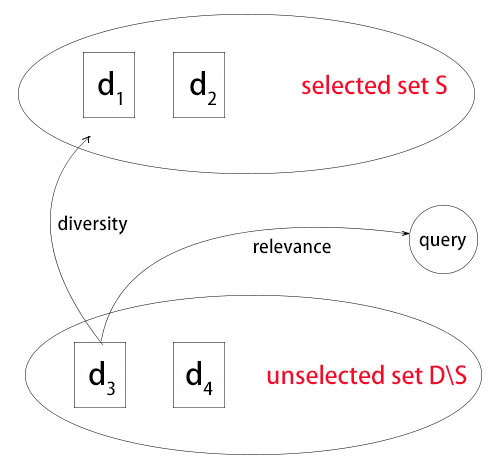
\includegraphics[width=0.65\textwidth]{fig_rank}
	\caption{An illustration for sequential selection in topic diversity model}
	\label{fig_rank}
\end{figure}

%In each step, we add the ``local-best" document with the highest score to the selected set.
\revised{
As for Eq. (\ref{eq1}), the left part corresponds to the relevance score and the right part corresponds to the diversity score. We look forward to redefine the estimation of diversity score $P(\bar{S}|q_i)$. According to the conditional probabilistic formula, the task can be formalized as follows: }
\begin{equation}
	P(\bar{S}|q_i)=\frac{P(\bar{S},q_i)}{P(q_i)}\overset{rank}{=}P(\bar{S},q_i)
	\label{eq3}
\end{equation}
where $P(q_i)$ denotes the occurrence rate of aspects $q_i$ corresponding to query $q$, which is usually regard to be normalized as 1/$n$  ($n$ denotes the number of aspects) \cite{santos2010exploiting}. Because the values of $P(q_i)$ are equal and do not impact on the result of ranking, we neglect $P(q_i)$.

%A Markov Random Field (MRF) is an undirected graphical model which possesses a set of random variables with Markov property. The MRF is used to model a joint probability distribution.
The main concern is how to define feature function for $P(\bar{S}, q_i)$. There are many ways to integrate different features, just like linear regression, logistic regression and some other ways. Under our situation, we use Markov Random Field (MRF) to model $P(\bar{S}, q_i)$. We benefit from its convenient combination of different types of features and we can get its derivation easily.

\subsection{Feature extraction via MRF}
A MRF is a probabilistic model defined on an undirected graph $G$. In MRF model, the nodes represent the random variables and the edges represent dependencies between these variables. In our study, the nodes represent the aspect $q_i$ and the unselected set $\bar{S}$. Consequently, we compute the joint probability defined over the graph $G$ as follows:
\begin{equation}
	P(\bar{S},q_i)=\frac{\prod_{l\in L(G)}\phi_l(l)}{Z},
	\label{eq4}
\end{equation}
where $L(G)$ is the cliques over the graph $G$, $\phi_l(l)$ is a potential function defined over the clique $l$, and $Z=\sum_{\bar{S}, q_i}\prod_l(l)$ is the normalization factor to ensure that $P(\bar{S}, q_i)$ satisfies a probability distribution.

The potential function is usually defined like:
\begin{equation}
	\phi_l(l)=exp(\lambda_lf_l(l)),
\end{equation}
where $f_l(l)$ is a feature function defined over clique $l$, and $\lambda_l$ is the corresponding weightiness factor. By applying log function and neglecting normalization factor, the final feature function is formalized as follows:
\begin{equation}
	P(\bar{S},q_i)\overset{rank}{=}\sum_{l\in L(G)}\lambda_lf_l(l).
	\label{eq9}
\end{equation}
Note that Eq. (\ref{eq9}) is derived from Eq. (\ref{eq4}) by neglecting the log function because its form is more simple for derivation and the simplifying does not impact the learning and ranking.
Nextly, we specify the structure of graph $G$ and its clique set $L(G)$ to derive our final feature functions.


\begin{figure*}[htb]
\centering
\subfigure[]
{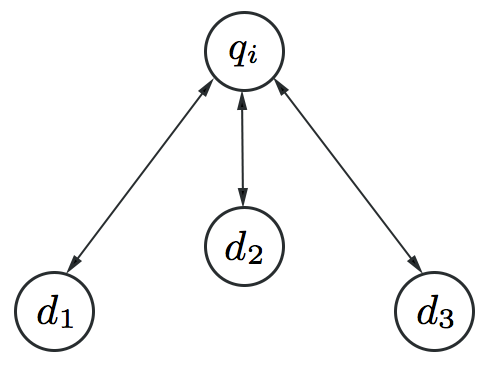
\includegraphics[width=0.32\textwidth]{fig1_1}}
\subfigure[]
{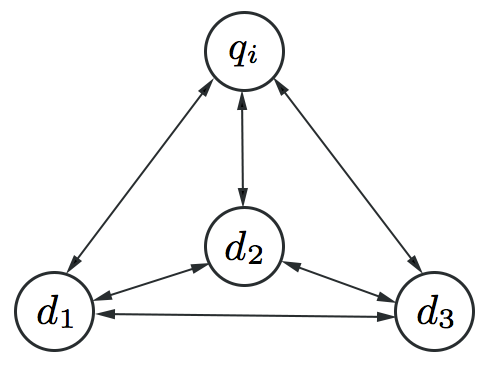
\includegraphics[width=0.32\textwidth]{fig1_2}}
\subfigure[]
{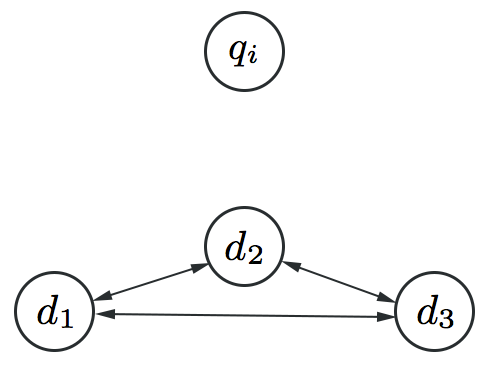
\includegraphics[width=0.32\textwidth]{fig1_3}}
\caption{An illustration for three types of cliques. The graph $G$ contains a aspects node $q_i$ and three document nodes (just for example) that correspond to the documents in the unselected set $\bar{S}$. (a) $l_{sd}$ contains $q_i$ and a single document node; (b) $l_{sD}$ includes $q_i$ and the whole $\bar{S}$; (c) $l_{D}$ only contains $\bar{S}$.}
\label{MRF}
\end{figure*}

Fig. (\ref{MRF}) shows the three types of cliques in MRF. The formal description about feature extraction based on three cliques is given as follows:
\begin{enumerate}
	%\item The $l_{sd}$. The high occupancy of aspects $q_i$ reflects the high potential relevance for $q_i$ with respect to $\bar{S}$. We define $f_{ave-topic}=ave_{d\in \bar{S}}dis(q_i, d)$, where dis(.,.) is the aspect distribution of document $d$ for topic $q_i$. Specially, we use $P(q_i|d)$ for our definition of $dis(q_i, d)$. $P(q_i|d)$ is the aspects distribution measurement.
	\item Based on $l_{sd}$. The high occupancy of aspects $q_i$ reflects the high potential relevance for $q_i$ with respect to $\bar{S}$.

		\begin{itemize}
			\item We define $f_{ave-topic}=ave_{d\in \bar{S}}P(q_i|d)$ for feature function on this clique. $P(q_i|d)$ is the aspects distribution measurement which we have mentioned in section \ref{mine_aspect}.
		\end{itemize}
	%\item The $l_{sD}$. The clique involves the inter-relationships in the candidate set $\bar{S}$. Correspondingly, we use the maximal, minimal, standard deviation of the $dis(q_i, d)_{d\in \bar{S}}$ as feature functions defined upon clique $l_{sD}$. For the sake of minimizing redundancy, we use the $num_{q_i}(\bar{S})-num_{q_i}(S)$ as a feature function defined on this clique too. $num_{q_i}(x)$ represents the number of documents in set $x$ with respect to aspects $q_i$.
	\item Based on $l_{sD}$. The clique involves the inter-relationships in the candidate set $\bar{S}$.
		\begin{itemize}
			\item We use the maximal, minimal, standard deviation of the $P(q_i|d)_{d\in \bar{S}}$ as feature functions defined upon clique $l_{sD}$.
			\item For the sake of minimizing redundancy, we use the $num_{q_i}(\bar{S})-num_{q_i}(S)$ as a feature function defined on this clique too. $num_{q_i}(x)$ represents the number of documents in set $x$ with respect to aspects $q_i$.
		\end{itemize}
	\item Based on $l_D$. Both $l_{sd}$ and $l_{sD}$ consider relations of documents with respect to the above two aspects. The clique $l_D$ only takes into account the relations among documents excluding aspects $q_i$. Previous research has shown that the aspect-independent property can indicate the relevance of documents for $q_i$ \cite{kurland2008rank}.
		\begin{itemize}
			\item We use the entropy of all the documents $d$ in $\bar{S}$: \\
$P_{entropy}(d)\overset{def}{=}-\sum_{w\in d}P(w|d)\log p(w|d)$ as feature function, where $w$ is a term and $p(w|d)$ is the probability that $w$ appears in $d$ (given by the language model).
			\item Spam ratio inspired by the Web Spam Classification is used for feature function, too \cite{fetterly2004spam}.
		\end{itemize}
\end{enumerate}


To conclude, by replacing the feature function into equation (\ref{eq1}) and putting the parameters $\lambda$ into the learning process, the ranking function is given as follows:
\begin{equation}
	f(d, \bar{S})=\lambda_rP(d|q)+\lambda_n\sum_{q_i\in Q}[P(q_i|q)P(d|q_i)\sum_{l\in L(G(q_i))}\lambda_lf_l(l)]
	\label{eq8}
\end{equation}
where $L(G(q_i))$ represents the clique set $L$ from the graph $G$ which is built around the aspects $q_i$, $f_l(l)$ stands for the feature function defined on the clique $l$. There exists a parameter $\lambda$ in equation (\ref{eq1}), it is a balance parameter between relevance and diversity. In our learning method, we use $\lambda_r$ and $\lambda_n$ to replace it and we can infer its value by learning process.



\subsection{Loss function}
% Given the precise definition of loss function, the next step is minimizing the loss function to get the best performance. Firstly, we generate the training data and apply the optimization method. Next, we use our ranking function to predict the final diverse ranking result.
%
% In this study, we use the data in TREC dataset in a format of quadruples: $(q^{(i)}, S^{(i)}, T_i, J(s_j^{(i)}|t_k))$, where $q^{(i)}$ means the i-th query $q$, $S^{(i)}$ is the corresponding related documents set, $T_i$ represent the sub-topic underlying the query $q^{(i)}$, and $J(s_j^{(i)}|t_k)$ represents the judgement factor whether the j-th document $s_j^{(i)}$ in $S^{(i)}$ covers the sub-topic $t_k$.
%
% Since the training data should be sorted according to the property of sequential selection, we construct a ideal ranked list $y_i$ which maximize the diversity metrics, such as $\alpha$-nDCG, ERR-IA, etc. In this study, we use metric ERR-IA to measure the results which is described as function $f_{ERR-IA}$. Algorithm \ref{ag1} is developed to construct a ideal ranked list, which is used to optimize the loss function. At the i-th step in algorithm \ref{ag1}, we select the document $d$ from $S\backslash X_{i-1}$ to maximize the function $f_{ERR-IA}$ and update the $S\backslash X_{i-1}$ by adding the document $d$. By recording the best document in every step, we get our final ideal ranked list as our training data.

We define the loss function as a likelihood loss of generation probability:
\begin{equation}
	L(rank(D, C), Y)=-\log P(Y|D),
	\label{eq6}
\end{equation}
where $rank$ denotes the ranking function in our model, $C$ is the feature function defined in unselected set $\bar{S}$, $D$ denotes all the candidate documents, and $Y$ is the final result of search result diversification. Because our L-SRD model is a sequential selection model, it can be viewed as maximizing probability of correctly choosing the top-n document from unselected set:
\begin{align}
	P(Y|D)&=P(y_1,y_2,...,y_n|D) \notag \\
		   &=P(y_1|D)P(y_2|D\backslash S_1)\cdots P(y_n|D\backslash S_{n-1}),
\end{align}
where $y_1,...,y_n$ is the ground truth for search result diversification task with respect to query $q$, $n$ represents the top $n$ result generated by the sequential selection process, the index $i$ denotes its ranking position, $S_{i-1}$ denotes the selected set after $i-1$ iterations, the probability $P(y_i|D\backslash S_{i-1})$ represents the probability that select the document $y_i$ under the condition of $D\backslash S_{i-1}$.

On the basis of the Plackett-Luce Model \cite{marden1996analyzing}, we derive the steps in our generation process shown as follows:
\begin{equation}
	%P(y_i|D\backslash S_{i-1})&=\frac{exp(f(y_i, D\backslash S_{i-1}))}{\sum_{k=i}^nexp(f(y_k, D\backslash S_{i-1}))}\\
P(Y|D)=\prod_{i=1}^nP(y_i|D\backslash S_{i-1})=\prod_{i=1}^n\frac{exp(f(y_i, D\backslash S_{i-1}))}{\sum_{k=i}^nexp(f(y_k, D\backslash S_{i-1}))},
	\label{eq7}
\end{equation}
% \begin{align}
% 	P(y_i|D\backslash S_{i-1})&=\frac{exp(f(y_i, D\backslash S_{i-1}))}{\sum_{k=i}^nexp(f(y_k, D\backslash S_{i-1}))}\\
% 	\label{eq7} P(Y|D)&=\prod_{i=1}^n\frac{exp(f(y_i, D\backslash S_{i-1}))}{\sum_{k=i}^nexp(f(y_k, D\backslash S_{i-1}))},
% \end{align}
where $S_0$ means empty set $\emptyset$, function $f$ corresponds to Eq. (\ref{eq8}). Incorporating Eq.(\ref{eq7}) into Eq.(\ref{eq6}), we get the definition of the loss function as follows:
\begin{equation}
	L(f(D, C), Y)=-\sum_{i=1}^n\log(\frac{exp(f(y_i, D\backslash S_{i-1}))}{\sum_{k=i}^nexp(f(y_k, D\backslash S_{i-1}))}).
\end{equation}


To get the final loss function, we simplify Eq. (\ref{eq8}) by uniting the parameter $\lambda_n$ and $\lambda_l$ (because the parameter in our model all can be decided by the learning process):
\begin{align}
	f(d, \bar{S})&=\lambda_rP(d|q)+\vec{\mu_d}\cdot N_{1...L}(d, q_i, \bar{S})\\
	N_l(d,q_i,\bar{S})&=\sum_{q_i\in Q}P(q_i|q)P(d|q_i)f_l(l)\ \ \ (l\in L(G(q_i)))
\end{align}
where $\vec{\mu_d}$ represents a L-dimensional weight vector, $L$ stands for the number of features, $N_{1...L}$ denotes a series of function vectors, $l$ is the cliques defined on $\bar{S}$ and $q_i$.

The total loss function is formulized as follows:
\begin{equation}
	-\sum_{i=1}^{T_r}\sum_{j=1}^{n}\log(\frac{exp(\lambda_rP(y_j|q)+\vec{\mu_d}\cdot N_{1...L}(y_j,q_i,\bar{S}))}{\sum_{k=j}^{n}exp(\lambda_rP(y_k|q)+\vec{\mu_d}\cdot N_{1...L}(y_k,q_i,\bar{S}))})
\end{equation}
where $T_r$ denotes the number of training examples.

\subsection{Learning and prediction}
Given the precise definition of loss function, the next step is minimizing the loss function to get the best performance. First, we generate the training data and apply the optimization method. Next, we use our ranking function to predict the final diverse ranking result.

In this study, we use the data in TREC dataset in a format of quadruples: $(q^{(i)}, RD^{(i)}, T_i, J(s_j^{(i)}|t_k))$, where $q^{(i)}$ means the $i$-th query $q$, $RD^{(i)}$ is the corresponding related documents set, $T_i$ represent the aspect underlying the query $q^{(i)}$ which are provided by official labeler, and $J(d_j^{(i)}|t_k)$ represents the judgement factor whether the j-th document $d_j^{(i)}$ in $RD^{(i)}$ covers the aspect $t_k$. Note that the last two elements in quadruples are used to calculate the score of evaluation metrics (e.g. $\alpha$-nDCG), we cannot make use of it directly in our model.

At first, we should generate a approximate ground truth for training set. So we construct a list $y_i$ which maximize the diversity metrics, such as $\alpha$-nDCG, ERR-IA, etc. In our study, we use ERR-IA to measure the results which is described as function $f_{ERR-IA}$. In algorithm \ref{ag1}, at the every $i$-th step in loop structure, we select the document $d$ from $D\backslash S_{i-1}$ to maximize the function $f_{ERR-IA}$ and update the $S\backslash D_{i-1}$ by adding the document $d$. By recording the best document in every step, we get our final ideal rankling list as our training data.


\begin{algorithm}[htb]
	\caption{Ideal ranking list construction algorithm}
	\begin{algorithmic}[1]
		\REQUIRE $(q^{(i)}, RD^{(i)}, T_i, J(d_j^{(i)}|t_k)), f_{ERR-IA}$
		\ENSURE $y_1,y_2,...,y_n$
		\STATE initialize $S_0=\emptyset$
		\FOR {$k=1$ to $n$}
		\STATE $bestDoc\leftarrow \arg\max_{d\in RD^{(i)}\backslash S_{k-1}}f_{ERR-IA}(d\cup S_{k-1})$
		\STATE $S_k=S_{k-1}\cup bestDoc$
		\STATE $y_k=bestDoc$
		\ENDFOR
	\end{algorithmic}
	\label{ag1}
\end{algorithm}

Nextly, we use the stochastic gradient descent method to optimize the loss function as shown in Algorithm \ref{ag2}. At every step in algorithm \ref{ag2}, we calculate the gradient according to Eq. (\ref{eq10})-(\ref{eq11}) and update the value of weight. The gradient in step $i$ at training set $D_{init}$ is computed as follows:
\begin{align}
	\Delta\lambda_r^{(i)}=\sum_{j=1}^{n}&(\frac{\sum_{k=j}^{n}P(y_j|q)exp(\lambda_r^{(i-1)}P(y_j|q)+\vec{\mu_d}^{(i-1)}\cdot N_{1...L}(y_j,q_i,\bar{S}))}{\sum_{k=j}^{n}exp(\lambda_r^{(i-1)}P(y_k|q)+\vec{\mu_d}^{(i-1)}\cdot N_{1...L}(y_k,q_i,\bar{S}))} \notag \\
	 &-\frac{P(y_j|q)exp(\lambda_r^{(i-1)}P(y_j|q)+\vec{\mu_d}^{(i-1)}\cdot N_{1...L}(y_j,q_i,\bar{S}))}{exp(\lambda_r^{(i-1)}P(y_k|q)+\vec{\mu_d}^{(i-1)}\cdot N_{1...L}(y_k,q_i,\bar{S}))})
	 \label{eq10}
\end{align}

\begin{align}
	\Delta\vec{\mu_d}^{(i)}=\sum_{j=1}^{n}&(\frac{\sum_{k=j}^{n}N_l(y_j,q_i,\bar{S})exp(\lambda_r^{(i-1)}P(y_j|q)+\vec{\mu_d}^{(i-1)}\cdot N_{1...L}(y_j,q_i,\bar{S}))}{\sum_{k=j}^{n}exp(\lambda_r^{(i-1)}P(y_k|q)+\vec{\mu_d}^{(i-1)}\cdot N_{1...L}(y_k,q_i,\bar{S}))} \notag \\
	&-\frac{N_l(y_j,q_i,\bar{S})exp(\lambda_r^{(i-1)}P(y_j|q)+\vec{\mu_d}^{(i-1)}\cdot N_{1...L}(y_j,q_i,\bar{S}))}{exp(\lambda_r^{(i-1)}P(y_k|q)+\vec{\mu_d}^{(i-1)}\cdot N_{1...L}(y_k,q_i,\bar{S}))})
	\label{eq11}
\end{align}

\begin{algorithm}[htb]
	\caption{Parameter learning algorithm}
	\begin{algorithmic}[1]
		\REQUIRE training data: $D_{init}^{Tr}, (y_1...y_n)^{Tr}$\\
		parameter: learning rate $\eta$, tolerate $\epsilon$
		\ENSURE $\lambda_r, \vec{\mu_d}$
		\STATE Initialize $\lambda_r, \vec{\mu_d}$
		\REPEAT
		\STATE $\lambda_r^{(0)}=\lambda_r$, $\vec{\mu_d}^{(0)}=\vec{\mu_d}$
		\STATE Randomly choose one of the training data
		\FOR {$i=1,...,n$}
		\STATE Compute the gradient $\Delta\lambda_r^{(i)}$ and $\Delta\vec{\mu_d}^{(i)}$
		\STATE Update: $\lambda_r^{(i)}=\lambda_r^{(i-1)}-\eta\Delta\lambda_r^{(i)}$, $\vec{\mu_d}^{(i)}=\vec{\mu_d}^{(i-1)}-\eta\Delta\vec{\mu_d}^{(i)}$
		\ENDFOR
		\STATE $\lambda_r=\lambda_r^{(n)}$, $\vec{\mu_d}=\vec{\mu_d}^{(n)}$
		\UNTIL change for value of loss function below the tolerate $\epsilon$
	\end{algorithmic}
	\label{ag2}
\end{algorithm}


Finally, we propose a sequential prediction method as described in Algorithm \ref{ag3}. At the $i$-th step in algorithm \ref{ag3}, we select the best document $d$ from $D\backslash S_{i-1}$ to maximize our ranking score and update the candidate set $D\backslash S_{i-1}$ by adding document $d$. By recording the best document in every step, we predict the final diverse ranking list as result.

\begin{algorithm}[H]
	\caption{The prediction process}
	\begin{algorithmic}[1]
		\REQUIRE query $q$ and its retrieval result $D_{init}$, weight $\lambda_r$ and $\lambda_{nl}$
		\ENSURE $y_1,y_2,...,y_n$
		\STATE $S_0=\emptyset$
		\FOR {$i=1,...,n$}
		\STATE $best = \arg\max_{d\in D\backslash S_{i-1}}f(d, D\backslash S_{i-1})$
		\STATE $S_i=S_{i-1}\cup best$
		\STATE $y_i=best$
		\ENDFOR
	\end{algorithmic}
	\label{ag3}
\end{algorithm}


\section{Experiment}\label{sec_setup}
% In this section, we conduct extensive experiments to prove our L-SRD model outperform other search result diversification methods with respect to the evaluation metrics. Above all, we take a while to introduce the experiment setup.
%
% To verify the effectiveness of the L-SRD model, we conduct extensive experiments by comparing L-SRD method and several well-known baseline methods.


\subsection{Dataset and evaluation metrics}
There are 150 queries in our query set, from TREC web track 2009 (WT2009) \cite{clarke2009preliminary}, WT2010, WT2011(50 for each). Evaluation is done on the ClueWeb09 Category B retrieval collection\footnote{http://www.lemurproject.org/clueweb09.php/}. The collection consists of nearly 50 millions web pages in English. There is a list of aspects for each query with binary relevance judgements, which are provided by TREC assessors.
%The goal of diversity task in TREC web track is providing a sorted document list that maximize the coverage of the aspects underlying a query. The krovetz stemmer and stopword removal are applied both in the index and retrieval time.
%Our query set contains of 150 queries, from TREC web track 2009 (WT2009) \cite{clarke2009preliminary}, TREC web track 2010 (WT2010), TREC web track 2011 (WT2011) (50 for each). Evaluation is done on the ClueWeb09 Category B retrieval collection\footnote{http://www.lemurproject.org/clueweb09.php/}.

%As illustrate in Figure \ref{fig3}, there is a query with 5 aspects and their respective explainations. Empirically, each query is consist of 3-8 aspects, which are identified by TREC assessors. For instance, the query "horse hooves" is inputted as a test case. In order to conform to reality as far as possible, we cannot utilize the official aspects directly, which we explain it in next section.

% \begin{figure}[htb]
% \centering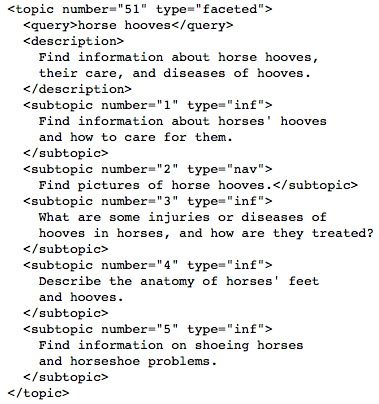
\includegraphics[width=0.45\textwidth]{fig2}
% \caption{TREC 2010 Web track, query 1, along with its corresponding aspects and explainations}
% \label{fig3}
% \end{figure}

%\subsection{Evaluation metrics}



\revised{
	There are three mainly evaluation metrics we use to evaluate the performance of our method: $\alpha$-nDCG \cite{clarke2008novelty}, ERR-IA \cite{chapelle2009expected}, NRBP \cite{clarke2009effectiveness}. 
	$\alpha$-nDCG is used to balance both relevance and diversity of candidate documents. ERR-IA measures the expected effort required for a user to satisfy their information needs. And NRBP is a feasible metric to evaluate the balance between the complexity of needs and the query.
	These metrics penalize redundancy in a different degree for the document at each sorted position to maximize the aspects coverage. Additionally, we report our result using Precision-IA  and Aspect Recall too. To measure the robustness, we use Win/Loss ratio metrics \cite{yue2008predicting,dang2012diversity}. The Win/Loss ratio denotes whether the model improve or hurt the result when comparing with the basic relevant baseline QL in terms of evaluation metrics \cite{dang2012diversity}. Particularly in our experiment, we use ERR-IA to calculate the Win/Loss ratio.
	}


%215 revised
\revised{
	The evaluation metrics are reported at different cutoffs. We use \{5, 10, 20\} as our cutoffs to set up experiments. These cutoffs focus on the evaluation at early ranking, which are particularly important in a Web search context \cite{jansen1998real}. The $\alpha$ is set to 0.5 in our experiments for the reason it gives equal weight to both relevance and diversity.
	}

\subsection{Baseline methods}\label{baseline_setting}

\revised{
We use the Indri\footnote{http://www.lemurproject.org/indri.php} to conduct our retrieval experiments and run with its default parameters configuration. %First, We generate three initial documents $D_{init}$ by three weighting models: language model (LM) \cite{hiemstra2001using}, BM25 \cite{robertson1995okapi} and TFIDF. And then, we employ these models with its default suggestion parameter settings: $ b $=0.75 in BM25, $\lambda_{LM}=0.15$ in LM.
All of the search result diversification methods are applied based on the top-$ K $ retrieved documents. As for the parameter $K$, we conduct a series of tests to find the appropriate $K$ maximizing the performance, which found 50 achieves the best result.}
%We use the Indri\footnote{http://www.lemurproject.org/indri.php} to conduct our retrieval run. All of the search result diversification methods are applied based on the top-K retrieved documents. As for the parameter $K$, we conduct a series of tests to finding the appropriate $K$ maximizing the performance, which found 50 achieves the best result.

Besides the baseline retrieval models, we compare L-SRD with some advanced diversification models as follows:
\begin{itemize}
    \item \textbf{QL}. The Query-likelihood language model is used for indri search engine as an initial retrieval method. We use it to provide the initial top 1000 documents for our diversification method. We also use it as a baseline method \cite{dang2012diversity}.
    
	\item \textbf{MMR}. A classical implicit diversification model. It is a representation of comparison between implicit and explicit models\cite{carbonell1998use}.
	
	\item \textbf{xQuAD}. xQuAD is a popular explicit diversification model which focuses on the redundancy of aspects \cite{santos2010exploiting}.
	
	\item \textbf{PM2}. PM2 is a popular explicit diversification model. PM2 generates the result set according to the aspects proportionality \cite{dang2012diversity}.
	
    \item \textbf{SVMDIV}. SVMDIV is also a learning model for search result diversification \cite{yue2008predicting}. It uses the structural SVMs to optimize the aspects coverage problem. But it only models the diversity without consideration of relevance. We get the source code from the svmdiv homepage\footnote{http://projects.yisongyue.com/svmdiv/} provided by the author.
    
    \revised{
    	\item \textbf{HxQuAD} is a hierarchical diversification model based on xQuAD \cite{Hu15searchresult}.
    	}
    
    \item \textbf{SMWE} mines query subtopic by exploiting the word embedding and short-text similarity measure. \cite{Ullah2016QuerySM}
\end{itemize}


%line 245
\revised{
These baselines 2-4 (corresponding to MMR, xQuAD, PM2) possess a single parameter $\lambda$ to tune, we perform a 5-fold cross validation to train $\lambda$ through optimizing ERR-IA. In our model, we use a 5-cross validation with a ratio of 3:1:1 for training, validation and prediction for the test query on each year. The final results are calculated over all the folds.}

%We use query suggestion method to generate the aspects underlying the query and re-submit the aspects to the search engine to get the aspect distribution $P(q_i|d)$ of aspect $q_i$ for document $d$, which is corresponding with \cite{santos2010exploiting}.

%\section{Experimental results}\label{sec_expres}
\subsection{Experimental results}\label{sec_expres}
%In this section, we evaluate L-SRD and the impact of critical step in it. To answer the questions in Section 4, we organise this section as follows. In Section 5.1, we investigate the impact of number of aspects generated in L-SRD and conduct a experiment based on standard metrics to make a comparison between L-SRD and other state-of-the-art search result diversification models in their best-case scenario. We emphasize the robustness of L-SRD by comparing it in different situations in Section 5.2. We divide it into three small sections, which respectively investigate the impact of different aspects generation approaches, the Win$\backslash$Loss ratio, and the result based on different retrieval models. At end, we discuss the time complexity of L-SRD in detail.
In particularly, our experiments aim to answer two main questions:

\begin{enumerate}
\item Can we utilize learning mechanism to promote the performance of search result diversification?
%\item To get a more stable performance, is it the implicit (e.g. topic model) or explicit (e.g. query logs) aspects generation way perform better?
\item Does L-SRD achieve better performance in terms of robustness comparing to other search result diversified models?
\end{enumerate}

%In this section, we evaluate L-SRD and the impact of critical step in it. To answer the questions, we organise this section as follows. We compare our model with other diversification models at section \ref{diver_com}. We emphasize the robustness of L-SRD in different situations in Section \ref{robut_anly}.

% \begin{figure*}[htb]
% \centering
% \subfigure[ERR-IA]
% {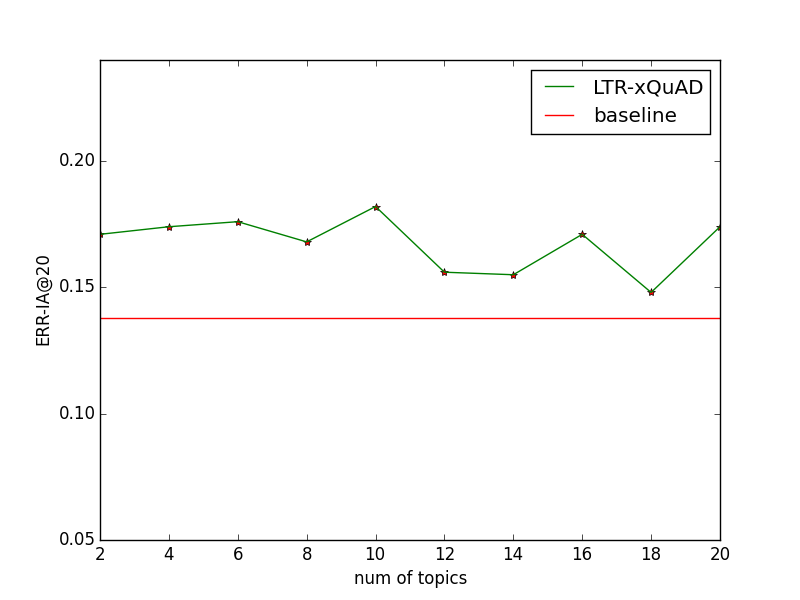
\includegraphics[width=0.43\textwidth]{fig4}}
% \subfigure[$\alpha$-nDCG]
% {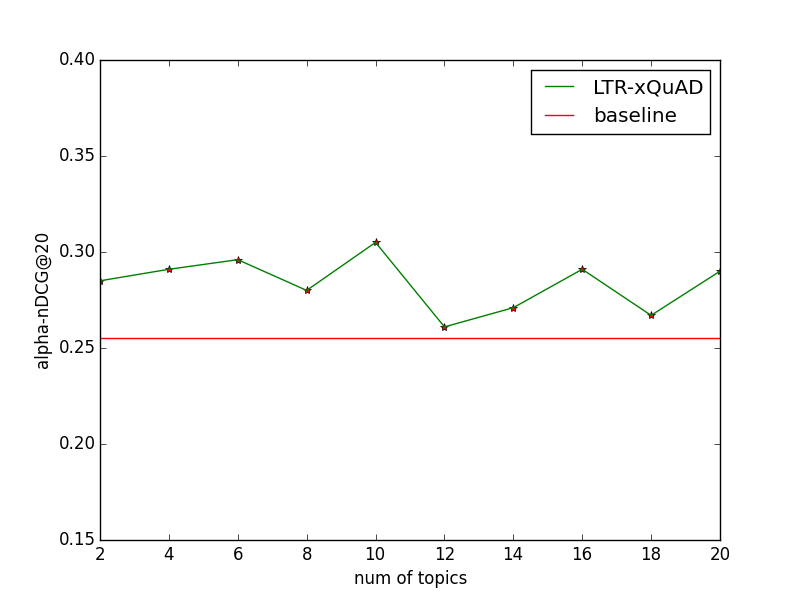
\includegraphics[width=0.43\textwidth]{fig6}}
% \subfigure[P-IA]
% {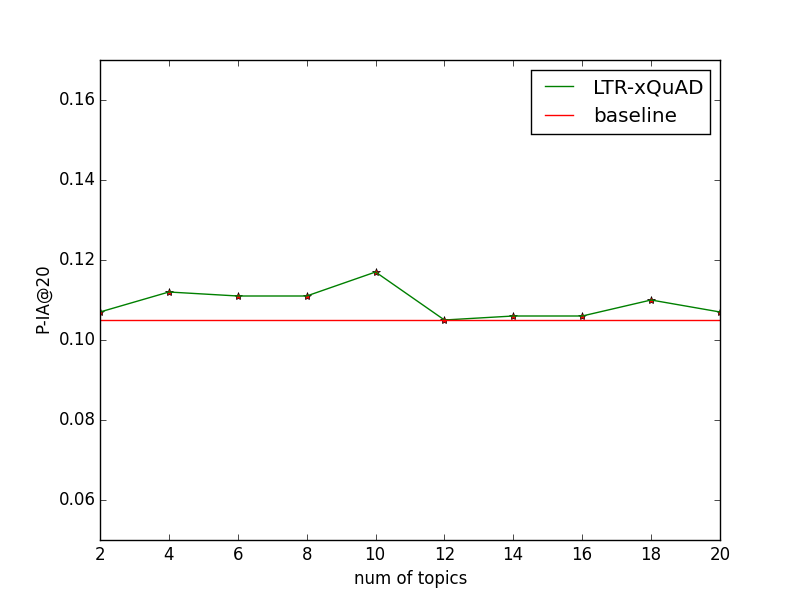
\includegraphics[width=0.43\textwidth]{fig7}}
% \caption{Comparing when varying number of latent topics used in our L-SRD model}
% \label{fig5}
% \end{figure*}
%
% \subsection{Tuning number of latent topics}
% Firstly, there also exisits a variable parameter in L-SRD, which is introduced by the step of aspects generation. We have to preset the number of topics to carry out the next latent topic inference approach. This parameter cannot be put into the learning approach, so we have to design a experiment to find out the most suitable number $LT$ (which means latent topics), and plot the result in Figure \ref{fig5}. We conduct our experiment in TREC web track 2009 (WT2009) in terms of three diversity metrics: ERR-IA, $\alpha$-nDCG and P-IA. The figure illustrates that too little and too much topics both hurt the result in some degree. From the point of mathematical implication, the model with too little topics cannot categorize the documents well, while the model with too much topics split the documents belong to the same category originally. They all hurt the performance of redundancy and proportionality measuring. According to our experiment, $LT = 10$ leads to the best result.

\subsubsection{Diversification analysis}\label{diver_com}
To answer question 1, we compare our L-SRD with other diversification models in terms of diversification metrics. Table \ref{tab1} shows the result of the evaluation in terms of $\alpha$-nDCG, ERR-IA, and NRBP. The best result per line is highlighted in bold. The classical MMR method is used as a representative of implicit diversification model \cite{carbonell1998use}. As for explicit model, we consider xQuAD and PM2 \cite{santos2010exploiting,dang2012diversity}. SVMDIV is selected for the representative of learning methods, HxQuAD is selected for the hierarchical model.

The result shows that L-SRD always performs best in terms of all metrics as shown in Table \ref{tab1}. It consistently improves the initial retrieval ranking method with gains up to \revised{23.19\%, 31.17\%, 15.11\%} in terms of $\alpha$-nDCG on WT2009, WT2010, WT2011 respectively. It indicates that our learning approach tackles the diversity measurement problem more effectively with the consideration of integrate different features. The reason is that features such as query-aspects relevance and information richness conform to the property of diversity. Furthermore, comparing with the explicit diversification models in terms of the evaluation of $\alpha$-nDCG, the improvement of L-SRD over the xQuAD is up to \revised{28.44\%, 16.87\%, 14.90\%} on WT2009, WT2010, WT2011 respectively, and the improvement of L-SRD over the PM2 is up to \revised{14.15\%, 23.11\%, 14.65\%} on WT2009, WT2010, WT2011 respectively. Previous explicit diversifications use a predefined function to calculate the diversity score, which cannot reach an optimal result from the overall situation. A learnable approach to solve the diversity measurement and parameter tuning problem is significative. 
\revised{
	In addition, comparing with the hierarchical diversification model in terms of the evaluation of $\alpha$-nDCG, the improvement of L-SRD over the HxQuAD is up to \revised{3.77\%, 9.68\%, 5.49\%} on WT2009, WT2010, WT2011 respectively. HxQuAD only use a predefined function to measure the diversity score, and the parameters may not be optimal because it needs to be tuned manually. Our learning model tackles the parameters tuning problem in an automatic fashion and reaches optimal result.
	Comparing with SWME in terms of the evaluation of $\alpha$-nDCG, the improvement of L-SRD over the HxQuAD is up to \revised{3.63\%, 5.35\%, 3.86\%} on WT2009, WT2010, WT2011 respectively. SMWE mines enough subtopics, but it cannot learn enough features to represent the document.
	}Besides the non-learning model, the improvement of L-SRD over the SVMDIV is up to 10.18\%, 14.70\%, 11.09\% on WT2009, WT2010, WT2011 respectively. It shows that considering relevance and different types of features in diversity measurement is helpful in the learning approach. That is the reason why our model wins. %The fact confirms that there exists a gap between utilizing the predefined diversity measure function and introducing feature learning approach in other side.
%The experimental data confirms that our method not only performs better than existing explicit diversification methods but also performs better than the existing learning method.
Therefore, L-SRD shows better understanding on the diverse ranking and leads to a better result. So we find that utilizing learning mechanism indeed promotes the performance of search result diversification.

\begin{table}[!htb]
\centering
%\small
%\tbl{Diversification performance using the official evaluation metrics for WT2009, WT2010, WT2011\label{tab1}}{%
\begin{tabular}{|c|c|c|c|c|}
\hline
Year & experiment & ERR-IA@20 & $\alpha$-nDCG@20 & NRBP \\%& P-IA@20\\
\hline
\multirow{6}{*}{2009}          & QL     & 0.1376          & 0.2548          & 0.1008          \\
					           & MMR    & 0.1405          & 0.2526          & 0.1070          \\
	                           & xQuAD  & 0.1411          & 0.2444          & 0.1113          \\
	                           & PM2    & 0.1482          & 0.2750          & 0.1101          \\
							   & SVMDIV & 0.1531          & 0.2849          & 0.1219          \\
							   & HxQuAD & 0.1653          & 0.3025          & 0.1372          \\
							   & SMWE   &  0.1787         & 0.3029          & 0.1482          \\
                               & L-SRD  & \textbf{0.1862} & \textbf{0.3139} & \textbf{0.1615} \\
\hline            
\multirow{6}{*}{2010}          & QL     & 0.1484          & 0.2445          & 0.1092          \\
	                           & MMR    & 0.1494          & 0.2450          & 0.1129          \\
	                           & xQuAD  & 0.1732          & 0.2746          & 0.1326          \\
                               & PM2    & 0.1599          & 0.2605          & 0.1175          \\
							   & SVMDIV & 0.1698          & 0.2796          & 0.1158          \\
							   & HxQuAD & 0.1807          & 0.2924          &  0.1303         \\
							   & SMWE   & 0.2038          &  0.3044          & 0.1601         \\
                               & L-SRD  & \textbf{0.2193} & \textbf{0.3207} & \textbf{0.1826} \\
\hline
\multirow{6}{*}{2011}          & QL     & 0.3288          & 0.4454          & 0.2802          \\
	                           & MMR    & 0.3253          & 0.4337          & 0.2834          \\
	                           & xQuAD  & 0.3235          & 0.4462          & 0.2812          \\
                               & PM2    & 0.3316          & 0.4472          & 0.2831          \\
							   & SVMDIV & 0.3429          & 0.4615          & 0.2923          \\
							   & HxQuAD & 0.3606          & 0.4860          & 0.3107          \\
							   & SMWE   & 0.3924          & 0.4936          & 0.3232         \\
                               & L-SRD  & \textbf{0.4078} & \textbf{0.5127} & \textbf{0.3374} \\

\hline
\end{tabular}
\caption{Diversification performance using the official evaluation metrics for WT2009, WT2010, WT2011}
\label{tab1}
\end{table}

We consider not only the advanced diversity metrics, but also traditional diversity metrics, such as Precision-IA and Aspect Recall. The former indicates how many relevant documents for each aspect we have for reranking, the latter indicates how many of the aspects for which we have relevant documents. The result is shown in Fig. \ref{fig4}. MMR still underperforms all of them, as for Precision-IA, xQuAD wins on WT2010 casually, while L-SRD performs more stable, even on WT2010, the gap is small. It proves that L-SRD outperforms others from different perspectives. Our learnable model solves the diverse ranking problem in a global perspective and always reaches prominent results.

\begin{figure}[htb]
\centering
\subfigure[Precicison-IA evaluation]
{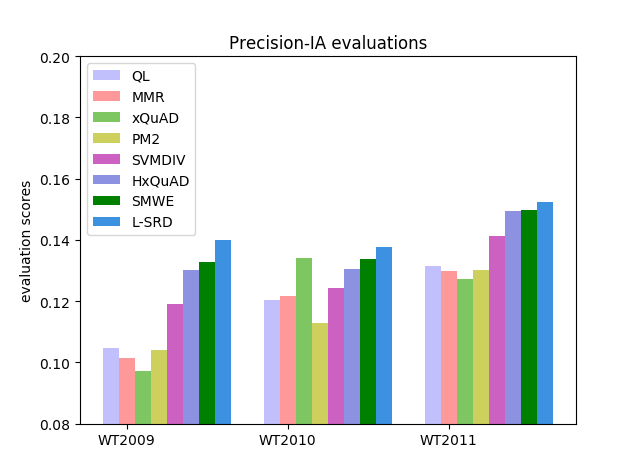
\includegraphics[width=0.47\textwidth]{paper1_pre}}
\subfigure[Aspect Recall evaluation]
{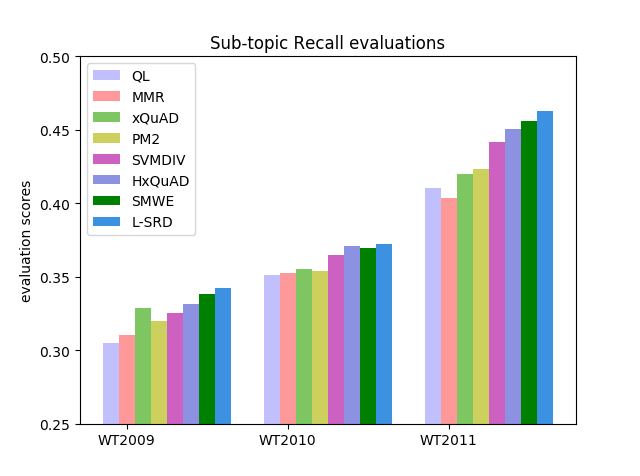
\includegraphics[width=0.47\textwidth]{paper1_sub}}
\caption{Performance comparison in WT2009, WT2010, WT2011 with Precision-IA and Aspect Recall}
\label{fig4}
\end{figure}

%\subsection{Experiment on the number of topics}


\subsubsection{Robustness analysis}\label{robut_anly}
%For the robustness analysis which we raise question 2,
An effective search result diversification method should not only outperform other models in terms of diversity metrics, but also maintain a high level of robustness, which we have raised the question 2.
We set up series of experiments on robustness research to study the Win/Loss behaviour and the usage of different retrieval algorithms respectively.

%An effective search result diversification model should not only outperform other models in some circumstances, but also possess a high level of robustness, which we have raised the question 2. To answer our question, we plan to set up series of investigation on robustness research. The investigation of robustness may be wide-ranging generally, so we divide our experiments into two sections, which discuss the Win$\backslash$Loss behaviour and different retrieval algorithms respectively.

% \subsubsection{aspects generation}
% At first, let us focus on the aspects generation. As we discussed above, there are two primary ways to generate the aspects. We have tested two way in xQuAD, PM2 and L-SRD in table \ref{tab2}, and find that the topic model (refer in particular to LDA \cite{blei2003latent} in our paper) performs more stable than the query suggestion model \cite{santos2010exploiting}. The query suggestion model are built with the help of Google index. We use subscript $LDA$ and $sug$ to identify two ways. It can be seen that in most cases the model based on LDA outperforms which based on query suggestion, even in the bad cases, the gap is small comparing with the good cases.
%
% From the point of resource utilization, the query suggestion way usually utilize the external resource (for instance, query logs) to mine the aspects underlying the query \cite{dang2012diversity,santos2010exploiting}, while LDA just extract the aspects from the perspective of semantic approach. The LDA reduces the expenses for collecting external resources and do well in our evaluation, that is the reason why we choose the LDA (latent dirichlet allocation) \cite{blei2003latent}, a classical topic model, to infer latent topics from a set of documents. Moreover, the experimental result answers the question 2 in Section 4.
%
%
% \begin{table}[htb]
% \centering
% %\tbl{aspects generate based on query suggestion and topic modeling\label{tab2}}{%
% \begin{tabular}{|c|c|c|c|}
% \hline
% Year & experiment & ERR-IA@20 & $\alpha$-nDCG@20\\
% \hline
% \multirow{6}{*}{2009}    & $xQuAD_{LDA}$   & 0.1411          & 0.2444\\
%                          & $xQuAD_{sug}$   & 0.1375          & 0.2547\\
% 	                     & $PM2_{LDA}$     & 0.1482          & 0.2750\\
%                          & $PM2_{sug}$     & 0.1321          & 0.2519\\
%                          & $L-SRD_{LDA}$ & \textbf{0.1862} & \textbf{0.3139}\\
%                          & $L-SRD_{sug}$ & 0.1807          & 0.3068\\
% \hline
% \multirow{6}{*}{2010}    & $xQuAD_{LDA}$   & 0.1732          & 0.2746\\
%                          & $xQuAD_{sug}$   & 0.1497          & 0.2468\\
%                          & $PM2_{LDA}$     & 0.1599          & 0.2605\\
%                          & $PM2_{sug}$     & 0.1636          & 0.2692\\
%                          & $L-SRD_{LDA}$ & 0.2193          & 0.3207\\
%                          & $L-SRD_{sug}$ & \textbf{0.2199} & \textbf{0.3214}\\
% \hline
%
% \multirow{6}{*}{2011}    & $xQuAD_{LDA}$   & 0.3235          & 0.4462\\
% 					     & $xQuAD_{sug}$   & 0.3218          & 0.4347\\
%                          & $PM2_{LDA}$     & 0.3316          & 0.4472\\
%                          & $PM2_{sug}$     & 0.3321          & 0.4508\\
%                          & $L-SRD_{LDA}$ & \textbf{0.4078} & \textbf{0.5127}\\
%                          & $L-SRD_{sug}$ & 0.3982          & 0.5039\\
% \hline
% \end{tabular}
% \caption{aspects generate based on query suggestion and topic modeling}
% \label{tab2}
% \end{table}

\begin{table}[!htb]
\centering
\begin{tabular}{|c|c|c|c|}
\hline
experiment & WT2009         & WT2010         & WT2011         \\
\hline
MMR        & 20/18          & 24/17          & 23/16          \\
xQuAD      & 23/18          & 23/16          & 24/14          \\
PM2        & 22/20          & 26/14          & 25/14          \\
SVMDIV     & 24/18          & 27/13          & 27/13          \\
HxQuAD     & 27/15          & 30/10          & 31/10          \\
SMWE       & 27/14          & 29/11          & 32/11          \\
L-SRD      & \textbf{28/14} & \textbf{30/10} & \textbf{32/10}  \\
\hline
\end{tabular}
\caption{Win/Loss ratio}
\label{tab3}
\end{table}

%\subsubsection{Win/Loss ratio}


%From the table \ref{tab3}, we find that our $L-SRD$ model performs best with its ratio of 2.65. It reflects the remarkable robustness of our model comparing with other outstanding diversification models. And it confirms the overall performance of our model is not restricted to a small subset, it still work in the whole dataset. Our introducing different type of features and learning approach address this problem well enough.

From table \ref{tab3}, we find that L-SRD model performs best with its ratio of 2.65. While the Win/Loss ratio of MMR, xQuAD, PM2, SVMDIV, HxQuAD and SMWE is 1.31, 1.46, 1.52, 1.77, 2.51, 2.44 respectively. It reflects the remarkable robustness of L-SRD model comparing with other outstanding diversification models. The promotion of robustness over the MMR, xQuAD, PM2 , SVMDIV, HxQuAD and SMWE is up to 102.28\%, 81.51\%, 74.34\%, 49.72\%, 5.58 \%, 8.61\% respectively. And it confirms the overall performance of our model is not restricted to a small subset, it still works in the whole dataset for three years data. Our different types of features and learning approach address this problem well.


\iffalse

\begin{table}[htb]
\centering
%\tbl{Results based on different retrieval model(as for WT2009)\label{tab4}}{%
\begin{tabular}{|c|c|c|c|c|c|c|}
\hline
& \multicolumn{3}{c}{$\alpha$-nDCG} & \multicolumn{3}{|c|}{ERR-IA}\\
\cline{2-7}
& @5 & @10 & @20 & @5 & @10 & @20\\
\hline
BM25     & 0.160          & 0.211          & 0.255          & 0.107          & 0.127          & 0.138\\
+MMR     & 0.188          & 0.216          & 0.256          & 0.124          & 0.136          & 0.145\\
+xQuAD   & 0.183          & 0.221          & 0.263          & 0.115          & 0.132          & 0.142\\
+PM2     & 0.174          & 0.209          & 0.252          & 0.108          & 0.124          & 0.135\\
+SVMDIV  & 0.193          & 0.246          & 0.285          & 0.128          & 0.141          & 0.153\\
+L-SRD & \textbf{0.242} & \textbf{0.268} & \textbf{0.314} & \textbf{0.161} & \textbf{0.174} & \textbf{0.186}\\
\hline
TFIDF    & 0.158          & 0.207          & 0.251          & 0.102          & 0.121          & 0.131\\
+MMR     & 0.173          & 0.215          & 0.259          & 0.118          & 0.126          & 0.135\\
+xQuAD   & 0.181          & 0.217          & 0.257          & 0.113          & 0.130          & 0.137\\
+PM2     & 0.189          & 0.223          & 0.263          & 0.117          & 0.133          & 0.142\\
+SVMDIV  & 0.187          & 0.238          & 0.279          & 0.119          & 0.136          & 0.148\\
+L-SRD & \textbf{0.237} & \textbf{0.255} & \textbf{0.302} & \textbf{0.151} & \textbf{0.169} & \textbf{0.180}\\
\hline
LM       & 0.095          & 0.147          & 0.195          & 0.054          & 0.074          & 0.085\\
+MMR     & 0.108          & 0.145          & 0.187          & 0.060          & 0.074          & 0.084\\
+xQuAD   & 0.099          & 0.159          & 0.199          & 0.056          & 0.078          & 0.088\\
+PM2     & 0.094          & 0.149          & 0.196          & 0.054          & 0.076          & 0.087\\
+SVMDIV  & 0.100          & 0.161          & 0.207          & 0.060          & 0.081          & 0.091\\
+L-SRD & \textbf{0.137} & \textbf{0.182} & \textbf{0.223} & \textbf{0.084} & \textbf{0.102} & \textbf{0.111}\\
\hline
\end{tabular}
\caption{Results based on different retrieval models (as for WT2009)}
\label{tab4}
\end{table}


%\subsubsection{Different retrieval algorithms}

%line 320
\revised{
Many retrieval algorithms can be used for providing search result from original input. As a concern for robustness, we look forward to investigate whether different retrieval algorithms affect the final result. In addition, we compare L-SRD with other search result diversification models by using different retrieval algorithms, such as BM25, TF-IDF, and Hiemstra's language modeling (LM). In particular, we employ the parameters setting as discussed in Section \ref{baseline_setting}.} 
%We evaluate the effectiveness of L-SRD on diversifying the search results produced by three effective probabilistic document weighting models: BM25, TF-IDF, and Hiemstra's language modelling (LM). }

%These weighting models are used to produce both a baseline ranking as well as the sub-rankings for different sub-queries. Additionally, we compare its performance to that of three diversification baselines.
%

Table \ref{tab4} shows the results of the robustness evaluation in terms of $\alpha$-nDCG and ERR-IA. Specially, L-SRD is the only approach continuously improving the evaluation result with respect to the baseline ranking methods. Our learnable model tackles the diversification problem with a global angle and adjusts the weight of parameters million times, so it performs more stable.
\fi


\section{Conclusion and Future Work}\label{sec_con}
In this paper, we propose a Learnable Search Result Diversification model (L-SRD). We pay our attention to the explicit Query Aspect Diversification models and introduce the learning approach to regard the model as a learning problem. Unlike the traditional explicit diversification models utilizing a predefined novelty measure function, we integrate different types of diversity features and estimate the weight with a learning approach. We derive our loss function as the likelihood of ground truth generation. Stochastic gradient descent algorithm is used to estimate the values of parameters. Benefiting from the learning approach, we can optimize the parameters in an automatic method. The prediction of our diversification model is provided by iterative maximizing the learned ranking function.

We have demonstrated the improvement of L-SRD comparing with other diversification models. We find L-SRD achieve considerable results in terms of official diversity metrics on three years in TREC web track dataset. To prove its robustness, we set the experiment about Win/Loss ratio and usage of different retrieval algorithms. We believe L-SRD will play an important role to improve the Query Aspect Search Result Diversification by using a learning method.

There exist a number of directions to be explored in the future. We look forward to take some considerable steps to make L-SRD achieve convergency as quick as possible. %Meanwhile, we desire to employ the learning approach on the hierarchical aspects underlying the query.

\section{Acknowledgments}


This research is supported by National Natural Science Foundation of China (Grant No. 61773229), Shenzhen Science and Technology Project (Grant No. CYZZ20150408152315667), Basic Scientific Research Program of Shenzhen City (Grant No. JCYJ20160331184440545), and Cross fund of Graduate School at Shenzhen, Tsinghua University (Grant No. JC20140001).


\section*{References}
%\bibliographystyle{splncs03}
%\bibliographystyle{model6-num-names}
%\biboptions{authoryear}
\bibliography{test}
\end{document}



\end{document}
